\documentclass[10pt]{article}

\usepackage[utf8]{inputenc}

\usepackage{titling}

\renewcommand{\tablename}{Tabla}
\renewcommand{\figurename}{Figura}
\renewcommand{\contentsname}{Contenidos}

\usepackage{hyperref}

% Remove the ugly borders around the links!
\hypersetup{
	pdfborder={0 0 0 [0 0]}
}

% Vertical bars
\usepackage{amsmath}

\usepackage{graphicx}
\graphicspath{{Img/}}

\usepackage{geometry}
\geometry{
	a4paper,
	left = 15mm,
	right = 15mm,
	top = 13mm,
}

\title{\textbf{Simulación de una red GSM}}
\author{Carlos Ortega Marchamalo \& Pablo Collado Soto \thanks{Proudly made with \LaTeX} \\ \\ \textbf{Conmutación} \\ \\ \textit{Universidad de Alcalá}}
\date{Mayo de $2020$}

\begin{document}
	\begin{titlingpage}
		\maketitle
		\vskip 3.5 cm
		\begin{figure}[!htb]
			\centering
			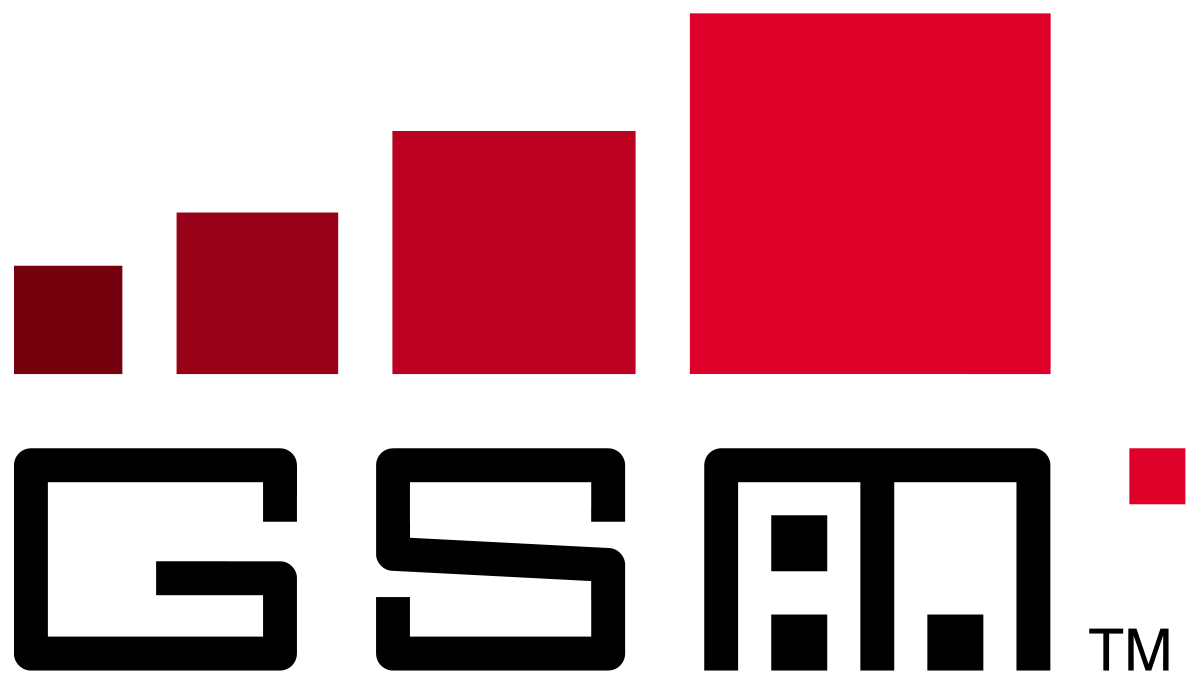
\includegraphics[width=0.75\linewidth]{GSM_logo.png}
		\end{figure}
	\end{titlingpage}

	\newpage
	\tableofcontents
	\newpage

	\section{Introducción}
		El paso del tiempo ha desencadenado cambios en muchos aspectos y ámbitos y las redes de comunicaciones no iban a ser menos. En un principio estas eran muy simples y rudimentarias y únicamente proporcionaban la conexión a teléfonos fijos. Sin embargo, los avances tecnológicos provocaron la aparición de dispositivos móviles que propiciaron modificaciones en las infraestructuras de telecomunicaciones hasta llegar al punto de nuestro interés y estudio: las redes \texttt{GSM}.

		La simulación de estos sistemas, tal y como ya hemos podido constatar, nos brinda nuevas posibilidades y nos permite reproducir el escenario que deseemos para corroborar la precisión y exactitud de los cálculos teóricos realizados previamente acerca de él así como apreciar posibles variaciones entre ambos procedimientos. Con este objetivo en mente partiremos de las nociones y conocimientos adquiridos en la parte teórica de la asignatura para, a partir de ellos, abordar los ya mencionados cálculos teóricos y posteriormente implementar el modelo en el simulador, analizando los resultados obtenidos a través de él y comparándolos con los extraídos con anterioridad.

		Así, en primer lugar llevaremos a cabo una breve explicación del sistema del que disponemos en su conjunto para proseguir con su análisis matemático, centrándonos, por un lado, en las llamadas y el bloqueo que estas sufren debido a las condiciones y circunstancias de la red existente y, desde otra perspectiva, examinando qué sucede en cuanto a los SMS y los retardos que padecen en función de las capacidades de los enlaces por los cuales transitan. Concluiremos plasmando todo esto en el \texttt{COMNET III}, teniendo que establecer ciertos ajustes para poder asimilar el esquema con la realidad a causa de ciertas carencias que este programa presenta.

		Esperemos haber sido capaces de plasmar esta información de una manera clara y concisa para así comprender de un mejor modo su contenido sin haber alcanzado el punto de la reiteración o complejidad en las descripciones elaboradas.

	\section{Un apunte sobre las redes \texttt{GSM}}
		A lo largo del documento aludiremos a entidades \texttt{GSM} de forma continuada. Es por ello que incluimos una breve relación de las mismas acompañada de alguna aclaración que facilite el seguimiento de nuestras explicaciones:

		\begin{itemize}
			\item \texttt{MS} (\textit{Mobile Station}): Equipo usuario de la red \texttt{GSM} que se compone de un terminal y una tarjeta \texttt{SIM}. Nosotros emplearemos los términos \texttt{MS} y \textit{usuario} de manera intercambiable ya que de cara a nuestro análisis estadístico son análogos.
			\item \texttt{BTS} (\textit{Base Transceiver Station}): Es la primera entidad funcional que se encuentra una \texttt{MS} al hacer uso de la red \texttt{GSM}. Su principal función es proveer a las \texttt{MS} de acceso a la red \texttt{GSM} a través de radioenlaces. Nosotros usaremos los términos \texttt{BTS} y \textit{célula} de manera intercambiable.
			\item \texttt{BSC} (\textit{Base Station Controller}): Estas entidades controlan los recursos radio de acceso a la red. Cada \texttt{BSC} controla varias \texttt{BTS} con lo que debemos ser conscientes de que también aglomeran el tráfico de varias estaciones base.
			\item \texttt{MSC} (\textit{Mobile Switching Center}): Esta entidad es el análogo a los conmutadores telefónicos de la red de telefonía fija y se encarga de cursar las llamadas desde las \texttt{MS} a las que sirve o hasta ellas. Al igual que ocurre con el par \texttt{BTS -- BSC} un \texttt{MSC} también tiene asociados varios \texttt{BSC} con lo que el tráfico cursado por un \texttt{MSC} es la superposición del cursado por los \texttt{BSC} a su cargo.
			\item \texttt{SMSC} (\textit{SMS Center}): Esta entidad se encarga de almacenar los mensajes \texttt{SMS} (\textit{Short Message Service}) hasta su entrega. De cara a nuestro cometido solo nos interesa saber que es el destino de los \texttt{SMS} enviados por nuestras \texttt{MS}.
		\end{itemize}

		Teniendo estos conceptos en mente podemos pasar a comentar la anatomía de nuestro sistema.

	\section{Descripción de la red estudiada}
		\subsection{Visión estructural}
			Antes de comenzar a observar más de cerca cada una de las aŕeas del sistema estudiado, hemos querido presentar un modelo general que nos permita ubicarnos en todo momento. Al analizar la probabilidad de bloqueo de las llamadas y los retardos sufridos por los \texttt{SMS} ahondaremos en las visicitudes de cada uno de los bloques estructurales de la red. Este "mapa" se puede consultar en la figura \ref{f:general_sys}. Con todo, pasamos a analizar desde un punto de vista teórico las diferentes partes del modelo.

			\begin{figure}
				\centering
				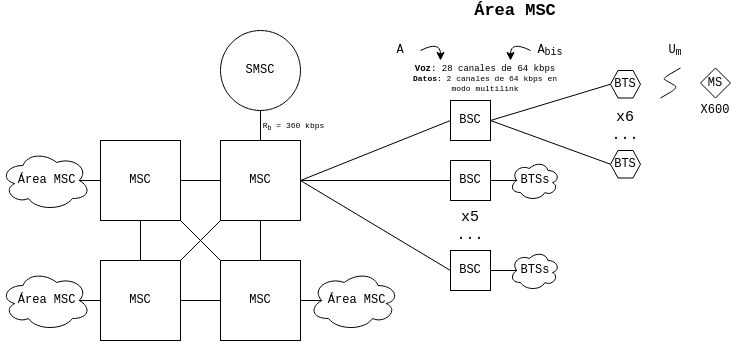
\includegraphics[width=1\linewidth]{GSM_system.png}
				\caption{Visión general del sistema estudiado.}
				\label{f:general_sys}
			\end{figure}

		\subsection{Características del tráfico y la red}
			Previo a la descripción del escenario debemos comentar las características del tráfico generado por los usuarios de la red. Cada \texttt{MS} hará en media $0,5\ \frac{llamadas}{h}$ con una duración esperada de $2\ min$. La señalización asociada a la llamada dura $8\ s$. Asimismo, cada terminal recibirá y enviará, en media, $1,25\ \frac{SMS}{h}$ y $1,75\ \frac{SMS}{h}$ respectivamente. Estos \texttt{SMS} tienen un tamaño fijo de $500\ B$ y su retardo de tránsito en la interfaz radio ($U_m$) es de $3\ s$. Todos los tiempos que se han proporcionado son medias y además se distribuyen exponencialmente. Esto es también cierto para el tiempo entre llegadas con lo que dichas llegadas seguirán un proceso de \textit{Poisson}. Esto nos permite modelar nuestros sistemas de manera que podamos aplicar sistemas de colas ya conocidos como son el $M/D/1$ y el $M/M/N/N$ según la notación de \textit{Kendall}.

			Además de lo anterior somos conscientes de que cada \texttt{BTS} sirve a $600\ MS$. Asimismo, cada célula cuenta con $14$ canales \texttt{TCH/H} que permiten cursar tráfico telefónico. Señalamos que la asignación de las células corresponde a un tráfico bajo y que se nos comunica que las combinaciones de tráfico son \texttt{C-II}, esto es, empleamos $14\ canales$ \texttt{TCH/H} en vez de $7\ canales$ \texttt{TCH/F}. La estrategia de asignación es temprana. Teniendo en cuenta el número de usuarios que pueden llegar a competir por estos canales asistiremos a una probabilidad de bloqueo que estudiaremos más adelante.

			Las interfaces $A_{bis}$ y $A$ que conectan a una \texttt{BTS} con un \texttt{BSC} y a un \texttt{BSC} con un \texttt{MSC} respectivamente se soportan sobre una portadora \texttt{E1} que cuenta con $30\ canales$ con una tasa $R_{ch} = 64\ kbps$ cada uno. Es por ello que cada canal de la portadora puede multiplexar $4\ llamadas$. Señalamos que en cada interfaz se reservan $2\ canales$ para cursar datos en vez de flujos de voz. En la sección pertinente comentaremos algo más acerca de la forma de explotar sendos canales.

			A la luz de estas características comenzamos nuestro estudio.

	\section{Probabilidad de bloqueo de las llamadas entre una \texttt{MS} y el \texttt{MSC} asociado}
		\subsection{Estudio teórico}
			Tal y como comentábamos en la sección anterior la estrategia de asignación de los canales \texttt{TCH} es temprana. Esto significa que podemos asumir que tanto la señalización asociada a la llamada como la propia voz discurren por este tipo de canal lógico, el \texttt{TCH}. En otras palabras, el bloqueo vendrá determinado por la disponibilidad de estos $14\ canales$ y no por aquellos dedicados a cursar única y exclusivamente señalización como son los \texttt{SDCCH}. Las implicaciones de esto no solo facilitan el análisis teórico del tráfico telefónico sino que además permiten compartimentar el estudio de este tráfico y el de datos.

			Con todo, si tenemos en cuenta el tráfico generado por cada usuario así como la duración de la llamada \textbf{y} el tiempo que toma la señalización obtenemos el tráfico de voz total que debe asumir cada \texttt{BTS}:

			$$A_{BTS} = N_{MS} \cdot \frac{\lambda_{MS}}{\frac{1}{T_{S_{TCH}}}} = 600\ MS\ \cdot\ \frac{0,5\ \frac{llamadas}{h} \cdot \frac{1\ h}{3600\ s}}{\frac{1}{120\ s\ +\ 8\ s}} = 10,67\ E$$

			Esta expresión nace de la propia definición de tráfico:
			
			$$A\ [E] = \frac{\lambda [\frac{llamadas}{s}]}{\mu [\frac{llamadas}{s}]} = \frac{\lambda [\frac{llamadas}{s}]}{\frac{1}{T_S [s]}}$$

			Recordamos que los datos anteriores se detallaban al comentar los aspectos generales del modelo. Dado el tamaño de nuestra población ($p = 600\ MS$) y teniendo en cuenta que el número máximo de llamadas que podemos cursar de manera concurrente es solo $14$, podemos asumir que nuestro sistema se comporta como un $M/M/N/N$. Tengamos en cuenta que $p \in [600 - 14,\ 600] \rightarrow p \in [586,\ 600]$. Dado lo reducido de este entorno de centro $593$ y radio $7$ podemos asumir que $p \approx cte$. Trabajar con este modelo facilitia la obtención de las probabilidades de bloqueo que nos interesan pues son el resultado de la función \textit{Earlang-B} con el tráfico soportado y el número de canales como entrada. En otras palabras, la probabilidad de bloqueo por falta de canales \texttt{TCH/H} en cada \texttt{BTS} viene dada por:

			$$P_{b_{U_m}} = E_1(A_{BTS}, N_{TCH/H}) = E_1(10,67\ E, 14\ TCH/H) = 0,075237 \rightarrow P_{b_{BTS}} = 7,5237\ \%$$

			Acabamos de obtener la probabilidad de bloqueo en solo el primero de los tres tramos que conectan a una \texttt{BTS} determinada con el \texttt{MSC} asociado, la interfaz radio $U_m$. Es por ello que debemos ver qué ocurre en las interfaces $A_{bis}$ y $A$.

			Tal y como hemos comentado estas dos últimas interfaces se soportan sobre $28\ canales$ de una portadora \texttt{E1}. Además cada canal puede multiplexar $4\ llamadas$ a su través lo que supone que, en total, estas interfaces pueden soportar $28 \cdot 4 = 112\ llamadas$ simultáneas. Si observamos la figura \ref{f:general_sys} nos daremos cuenta de que la interfaces $A_{bis}$ y $A$ se comparten entre las $8$ \texttt{BTS} a las que dan servicio. Como cada \texttt{BTS} solo es capaz de soportar $14\ llamadas$ en paralelo dada su asignación de canales \texttt{TCH/H} llegamos a la conclusión de que las $8$ \texttt{BTS} pueden suponer como máximo un total de $8 \cdot 14 = 112\ llamadas$ simultáneas también. Esto implica que \textbf{NO} existirá bloqueo de llamadas telefónicas en estas interfaces en ningún caso.

			Podemos pensar que son las \texttt{BTS} las que piden canales a estas interfaces y dado el límite que imponen los canales \texttt{TCH/H} vemos que nunca se solicitarán más canales de la portadora \texttt{E1} de los que se puedan suministrar. Esto ocurre siempre que el número máximo de llamadas a cursar por un enlace sea menor o igual que los canales del mismo.

			Si somos estrictos, la probabilidad de bloqueo de llamadas entre una \texttt{BTS} y un \texttt{MSC} ($P_{b_{BTS-MSC}}$) vendría dada por:

			\begin{equation}
				P_{b_{BTS-MSC}} = 1 - \prod_{i = 0}^N (1 - P_{b_i});\ donde\ N = 2\ y\ P_{b_0} = P_{b_{U_m}};\ P_{b_1} = P_{b_{A_{bis}}};\ P_{b_2} = P_{b_A}
				\label{eq:Pb}
			\end{equation}

			Teniendo en cuenta que tal y como comentábamos $P_{b_{A_{bis}}} = P_{b_A} = 0$ llegamos a:

			$$P_{b_{BTS-MSC}} = 1 - (1 - P_{b_{U_m}})(1 - 0)(1 - 0) = P_{b_{U_m}} = 7,5237\ \%$$

		\subsection{Corroboración con las simulaciones}
			Si bien la teoría que sustenta nuestros resultados es sólida debemos ver si las simulaciones de la red son congruentes con los resultados esperados. Tal y como venimos haciendo hasta ahora vamos a representar nuestro modelo a través de los nodos que nos ofrece el programa que emplearemos \texttt{COMNET III}.

			Al estar tratando con probabilidades de bloqueo optaremos por llevar a cabo una sola repetición del escenario con un tiempo tremendamente largo. Con ello buscamos conseguir un número de llamadas bloqueadas lo suficientemente elevado como para poder estar seguros de nuestros resultados. Dado que las probabilidades de bloqueo pueden oscilar entre el $0\ \%$ y el $100\ \%$ daremos por válidos aquellos resultados cuyo número total de llamadas bloqueadas sea igual o superior a $100$. No obstante, en busca de una mayor exactitud decidimos elevar el objetivo de llamadas bloqueadas para asegurar que los resultados de la simulación fueran los esperados.

			Con una repetición de $80000\ s$ de duración y un transitorio de $8000\ s$ (el $10\ \%$ del tiempo de la simulación) en el que no se consideraban las llamadas bloqueadas a fin de estudiar el sistema en su estado estacionario o regimen normal asistimos a una probabilidad de bloqueo del $7,2\ \%$ con $6602$ llamadas bloqueadas. Señalamos que esta probabilidad es muy cercana al $7,5237\ \%$ que habíamos augurado, con lo que podemos estar seguros de haber analizado el sistema correctamente.

			\subsubsection{Una nota sobre el modelado en \texttt{COMNET III}}
				Un aspecto del que debemos ser siempre conscientes es que a la hora de trabajar con programas de simulación debemos modelar los sistemas estudiados de la forma más fidedigna posible. No obstante, en ocasiones podemos darnos de bruces con infraestructuras tremendamente complejas con lo que deberemos ingeniárnoslas para que nuestra representación se ajuste a la realidad.

				En nuestro caso debemos replicar $8$ células para representar todas las \texttt{BTS} servidas por un mismo \texttt{BSC}. Pensando que quizá podría resultar muy tedioso además de poco manejable en el evento de tener que realizar cambios, nos propusimos representar una sola célula e "inyectar" de manera artificial el tráfico del resto de \texttt{BTS}. En las figuras \ref{f:full_bsc_area} y \ref{f:condensed_bsc_area} se pueden observar los modelos completo y condensado, respectivamente.

				\begin{figure}
					\centering
					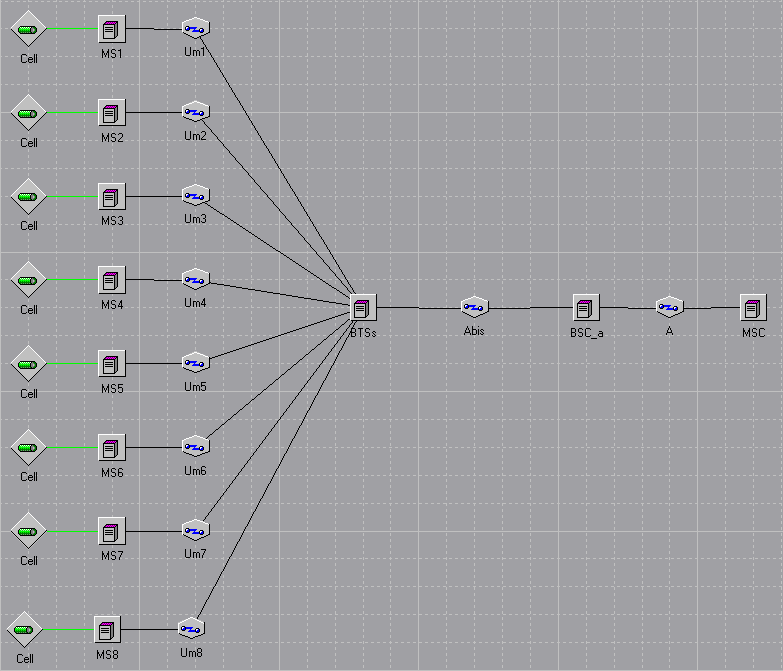
\includegraphics[width=0.5\linewidth]{full_bsc_area.png}
					\caption{Modelo completo del área de servicio de un \texttt{BSC}.}
					\label{f:full_bsc_area}
				\end{figure}

				\begin{figure}
					\centering
					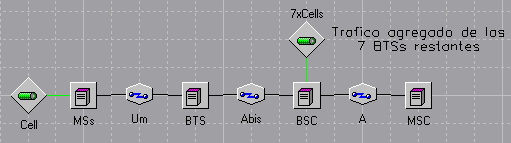
\includegraphics[width=0.5\linewidth]{condensed_bsc_area.png}
					\caption{Modelo "condensado" del área de servicio de un \texttt{BSC}.}
					\label{f:condensed_bsc_area}
				\end{figure}

				A pesar de que estos dos modelos parezcan idénticos no debemos pasar por alto la sutileza que supone que las \texttt{BTS} limiten el número de llamadas que se pueden cursar a su través de forma simultánea. Recordamos que cada \texttt{BTS} contaba con $14\ canales$ \texttt{TCH/H} lo que supone que solo se podían mantener $14\ llamadas$ simultáneamente en una célula. En última instancia esto implicaba que no existiría bloqueo en las interfaces $A_{bis}$ y $A$. Si condensamos el modelo "inyectando" tráfico de manera artificial veremos que esta restricción no se mantiene en las $7$ \texttt{BTS} que estamos representando con una fuente de mensajes común ya que no existe la limitación impuesta por el número finito de canales de tráfico. En un momento dado podríamos tener más de $14\ llamadas$ por \texttt{BTS} con lo que la probabilidad de bloqueo en las interfaces anteriores no sería nula. Tal y como demuestra la expresión \ref{eq:Pb} esto variaría la probabilidad de bloqueo pedida al ser $P_{b_{A_{bis}}} \neq 0$ y $P_{b_A} \neq 0$.

				Tal y como podríamos esperar, encontraremos probabilidades de bloqueo mayores de las esperadas al representar nuestro modelo de manera simplificada con lo que los datos aportados han sido obtenidos del modelo representado en la figura \ref{f:full_bsc_area}.

			\subsubsection{Comentarios finales sobre el bloqueo de llamadas}
				A lo largo de esta sección hemos comentado todos los aspectos realtivos al posible bloqueo de llamadas del sistema. Dado lo finito del espacio del que disponemos para realizar el informe hemos optado por redactar todos los hallazgos obviando algunas de las preguntas propuestas en el guión de la práctica. Hemos obrado así ya que sabiendo el resultado final podemos contestar a estas cuestiones sin lugar a dudas.

				En primer lugar vemos que tras modelar las interfaces $A_{bis}$ y $A$ la probabilidad de bloqueo permanece constante tal y como comentábamos. Asimismo, el cambiar la tasa binaria de los canales de voz de $64\ kbps$ a $16\ kbps$ no tiene impacto alguno sobre los resultados. De cara al análisis de las probabilidades de bloqueo estamos interesados en el número de canales que ocupa una llamada, no en su calidad. Así, como al modificar la tasa de los canales hacemos lo propio con la fuente de llamadas, los cambios se equilibran con lo que todo permanece igual. La diferencia entre ambos casos es la calidad de las llamadas, siendo la percibida por los usuarios en el contexto de $64\ kbps$ mayor.

				Con todo esperamos haber sabido puntualizar los aspectos más característicos del sistema sin que ello haya atentado contra la longitud o legibilidad de la sección. Es momento de estudiar el \textit{backbone} de datos sobre el que se soporta la infraestructura \texttt{SMS}.

	\section{Retardo medio de tránsito de los SMS entre una \texttt{MS} y el \texttt{SMSC}}
		\subsection{Estudio Teórico}
			Como ya hemos mencionado previamente, los dos ámbitos, el de las llamadas y el de los \texttt{SMS}, son independientes debido a que tanto el tráfico de voz como la señalización relacionada transcurren en su totalidad por los canales \texttt{TCH} en la interfaz radio pues se emplea una asignación temprana de recursos. De este modo, por los canales \texttt{SDCCH} solo viajarán los mensajes, los cuales se verán afectados por una probabilidad de bloqueo ya que la cantidad de canales radio no es suficiente para cursar todos los datos que le llegan. Aprovechamos para recordar que asumimos que tal y como se comenta la \texttt{MS} que envía el \texttt{SMS} cuyo retardo queremos obtener pertenece al \texttt{MSC} que está directamente conectado al \texttt{SMSC}.

			Con todo, teniendo en cuenta que cada céluda aglutina $600\ MS$, cursando cada una de media $3\ \frac{SMS}{h}$ en global considerando los que genera y los que recibe, los cuales consumen $3\ s$ sobre el \texttt{SDCCH}, obtenemos un tráfico en cada \texttt{BTS} de:

			$$A_{BTS} = N_{MS} \cdot \frac{\lambda_{MS_{SMS}}}{\frac{1}{T_{S_{SDCCH}}}} = 600\ MS\ \cdot\ \frac{3\ \frac{SMS}{h} \cdot \frac{1\ h}{3600\ s}}{\frac{1}{3\ s}} = 1,5\ E$$

			Con esto, nos encontramos ante un sistema $M/M/N/N$ sustentado sobre $4$ líneas, como corresponde a la asignación típica de tráfico bajo. Aplicando por consiguiente la función $Earlang-B$, observamos el oportuno resultado de todo ello:

			$$P_{b_{U_m}}\bigr\rvert_{SMS} = E_1(A_{BTS}, N_{SDCCH}) = E_1(1,5\ E, 4\ SDCCH) = 0,047957 \rightarrow P_{b_{BTS}} = 4,47957\ \%$$

			En consecuencia, no todos los \texttt{SMS} enviados por una MS pasarán a la interfaz $A_{bis}$ puesto que sufrirán la probabilidad de bloqueo calculada. Partiendo de los $1.75\ \frac{SMS}{h}$ enviados por cada \texttt{MS} aplicamos la probabilidad de bloqueo obtenida para llegar a la tasa \textit{real} de \texttt{SMS} que cada \texttt{MS} enviará:

			$$\lambda_{MS_{SMS}}\biggr\rvert_{real} = 1.75\ \frac{SMS}{h}\ \cdot\ (1\ -\ P_{b_{U_m}}\bigr\rvert_{SMS}) = 1.75\ \frac{SMS}{h}\ \cdot\ (1\ -\ 0,047957) = 1,666\ \frac{SMS}{h}$$

			Podríamos plantearnos qué sucedería con los mensajes que entran a las \texttt{MS} esto es, si padecerían la plasmada probabilidad de bloqueo. Sin embargo, se da un hecho que debemos tener muy presente y es que por la naturaleza de las interfaces $A_{bis}$ y $A$, estos son ciertamente \textit{full-duplex} y, por tanto, el tráfico que circula en un sentido no influye en el contrario. Esta es la verdadera razón por la que no tenemos que preocuparnos en ningún momento por lo que ocurrirá con los \texttt{SMS} que se adentran a las \texttt{MS}. En otras palabras, al comunicarnos que la interfaz $A_{bis}$ se soporta sobre un \texttt{E1} debemos tener en cuenta que \textit{cada sentido cuenta con su propia portadora}. Dado que este análisis se centra en el dominio de los datos podemos pensar que tanto el sentido ascendente como el descendente cuentan con su propio enlace con lo que no existe dependencia entre estos dos flujos de tráfico. Es por ello que, como solo debemos analizar el retardo de un \texttt{SMS} desde una \texttt{MS} hasta el \texttt{SMSC} podemos centrarnos en el tráfico de subida y obviar el de bajada una vez abandonamos la interfaz radio $U_m$. Tal y como se observa, esto se debe a que los canales \texttt{SDCCH} \textbf{sí} son compartidos por los \texttt{SMS} entrantes y salientes mientras que, como comentamos, esto no es cierto más allá de la \texttt{BTS}.

			El siguiente trayecto que deben atravesar los mensajes se trata de la interfaz $A_{bis}$. Para esta circunstancia sí que consideramos el tamaño de los \texttt{SMS}, siendo este $L_{SMS} = 500\ B$ y constante, significando lo último que estamos en esta ocasión ante un modelo $M/D/1$. También se nos señala que los dos canales dedicados a este fin, cuya tasa binaria es de $R_{ch} = 64\ kbps$, se explotan en modo \textit{multilink}. Por tanto podemos trabajar como si tuvieramos un único canal de tasa $R_{b_{real}} = 2\ \cdot\ 64\ kbps = 128\ kbps$. A modo de curiosidad señalamos que para explotar estos $2$ enlaces en modo \textit{multilink} los \texttt{SMS} han de "trocearse" para que cada fragmento pueda ser enviado en paralelo. En el otro extremo ambas partes se reensamblarán para que el mensaje siga su curso. Este detalle no es importante para nosotros ya que con saber la tasa binaria resultante a emplear es suficiente pero no por ello deja de ser interesante conocer la implementación real de estos sistemas.

			El referido enlace proporciona recursos a las $8$ \texttt{BTS} dependientes de un \texttt{BSC}, esto es, tenemos que emplear la suma de todo el tráfico y que se traduce en una tasa de:

			$$\lambda_{A_{bis}} = 8\ \cdot\ N_{MS}\ \cdot\ \lambda_{MS_{SMS}}\biggr\rvert_{real} = 8\ \cdot\ 600\ \cdot\ 1,666\ \frac{SMS}{h} \cdot \frac{1\ h}{3600\ s} = 2,22\ \frac{SMS}{s}$$

			Por su parte, la tasa de servicio, es decir, la inversa del tiempo de servicio, se calcula en función del tamaño de los mensajes y el régimen binario del enlace sobre el que transitan. Así, para este caso, llegamos a:

			$$\mu_{A_{bis}} = \frac{1}{T_{S}} = \frac{R_{b_{A_{bis_{real}}}}}{L_{SMS}} = \frac{128\ kbps}{500\ B\ \cdot 8\ \frac{b}{B}} = 32\ \frac{SMS}{s}$$

			Tras esto, obtenemos $\rho_{A_{bis}}$ como:

			$$\rho_{A_{bis}} = \frac{\lambda}{\mu} = \frac{2,22}{32} = 0,06942$$

			Podemos ya, por fin, estimar el retardo de tránsito en la interfaz $A_{bis}$. Teniendo siempre en cuenta que el enlace se modela como un sistema $M/D/1$ y los valores obtenidos justo en los pasos anteriores llegamos a:

			$$E[T_{A_{bis}}] = \frac{\frac{1}{\mu}}{1 - \rho} \cdot (1 - \frac{\rho}{2}) = 32,4156\ ms$$
			
			A continuación nos encontramos con la interfaz $A$, la cual es especial pues presenta las mismas características que $A_{bis}$ y, a pesar de lo que pudiéramos pensar, en ella no se formará cola alguna. Esta situación se da porque los \texttt{SMS} están "saliendo" de la interfaz $A_{bis}$ cuya tasa binaria es la misma que la de la interfaz $A$; recordemos que ambas se sustentan sobre los mismos canales de la portadora \texttt{E1}. Como el único tráfico que atravesará $A$ es aquel que proviene de $A_{bis}$ (esto es, $\lambda_A = \lambda_{A_{bis}}$) y no tenemos ninguna aportación de otras fuentes veremos que en este segundo enlace \textbf{no} tendremos en efecto ninguna espera. Si "nos ponemos en la piel de un paquete" nos daremos cuenta de que el tiempo que tardamos en atravesar la interfaz $A_{bis}$ es suficientemente largo como para que el paquete que estuviera esperando a ser transmitido por $A$ lo haya hecho por completo. A la luz de esta sutileza \textbf{no} es correcto modelar la interfaz $A$ como un sistema $M/D/1$. Sabiendo que el tiempo de espera en cola es de $0\ s$ el retardo por este enlace será solo el tiempo de servicio:
			
			$$E[T_A] = T_{S_A} = T_{S_{A_{bis}}} = \frac{1}{\mu_{A_{bis}}} = \frac{1}{32\ \frac{SMS}{s}} = 31,25\ ms$$

			Para concluir, los \texttt{SMS} alcanzan el \texttt{SMSC} por medio de una línea caracterizada por una tasa de $R_{b_{SMSC}} = 360\ kbps$ que interconecta esta última instancia con una de las \texttt{MSC} existentes. Es por esta razón que la tasa de tráfico que cursa es el conjunto del que recibe cada una de las \texttt{MSC}. De esta manera, tendremos:

			$$\lambda_{SMSC} = N_{MSC}\ \cdot\ N_{\frac{BSC}{MSC}}\ \cdot\ N_{\frac{BTS}{BSC}}\ \cdot\ N_{\frac{MS}{BTS}}\ \cdot\ \lambda_{MS_{SMS}}\biggr\rvert_{real} = 4\ \cdot\ 8\cdot\ 8\ \cdot\ 600\ \cdot\ 1,666\ \frac{SMS}{h} \cdot \frac{1\ h}{3600\ s} = 71,086\ \frac{SMS}{s}$$

			En cuanto al cálculo de la tasa de servicio, el procedimiento es idéntico al reflejado previamente aplicando los datos correspondientes. Con ello:

			$$E[T_{SMSC}] = \frac{\frac{1}{\mu_{SMSC}}}{1 - \rho_{SMSC}} \cdot (1 - \frac{\rho}{2}) \approx 32\ ms\ donde\ \mu_{SMSC} = \frac{R_{b_{SMSC}}}{L_{SMS}} = 90\ \frac{SMS}{S};\ \rho_{SMSC} = \frac{\lambda_{SMSC}}{\mu_{SMSC}} = 0,78984$$

			Si recordamos que tal y como se nos comunica el retardo medio de tránsito de un \texttt{SMS} en la interfaz radio $U_m$ es $E[T_{U_m}] = 3\ s$ llegamos a que el retardo medio de tránsito total de un \texttt{SMS} entre una \texttt{MS} y el \texttt{SMSC} es:

			$$E[T_{MS \rightarrow SMSC}] = E[T_{U_m}] + E[T_{A_{bis}}] + E[T_A] + E[T_{SMSC}] = 3\ s\ +\ 32,4156\ ms\ +\ 31,25\ ms\ +\ 32\ ms = 3,0957\ s$$

		\subsection{Comprobación con las simulaciones}
			Lo primero que hicimos fue cerciorarnos de haber calculado correctamente la probabilidad de bloqueo de los \texttt{SMS} ($P_{b_{U_m}}\bigr\rvert_{SMS}$) a través del modelo representado en la figura \ref{f:sms_pb}. Lo que hicimos fue configurar una tasa de llamadas igual a la de los \texttt{SMS} entrantes y salientes a la célula mientras limitábamos el número de canales a los $4\ SDCCH$ de los que disponemos. Con una iteración de $9000\ s$ con sus correspondientes $900\ s$ de transitorio obteníamos una probabilidad de bloqueo del $4,7\ \%$ con $4487\ SMS$ bloqueados. Al ser el resultado muy próximo al valor teórico esperado del $4,48\ \%$ nos reafirmamos en nuestos cálculos.

			\begin{figure}
					\centering
					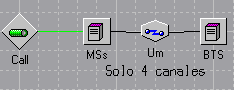
\includegraphics[width=0.3\linewidth]{sms_pb.png}
					\caption{Modelo para estudiar $P_{b_{U_m}}\bigr\rvert_{SMS}$}
					\label{f:sms_pb}
			\end{figure}

			Para verificar la validez de todos los retardos calculados anteriormente nos resuta muy valiosa la ayuda que nos proporciona el simulador \texttt{COMNET III}. Así, para extraer un análisis más consistente y preciso realizamos una prueba compuesta de $20$ iteraciones, cada una de las cuales tiene una duración de $600\ s$ y un transitorio de $60\ s$ que permite que las medidas tomadas puedan atribuirse al régimen permanente de operación. Esto es, las medidas que se nos proporcionan se toman en el intervalo $t \in [60,\ 660]\ s$. Al emplear $20$ iteraciones conseguimos una mayor precisión en los resultados ya que una mayor cantidad de muestras nos permiten acercarnos más a la media real del parámetro estudiado. Asimismo, estos intervalos de confianza se han calculado para $\alpha = 0,05$ o lo que es lo mismo, la media real se encontrará dentro de dicho intervalo con una probabilidad del $95\ \%$.

			Con estas condiciones obtenemos unos resultados que adjuntamos en la siguiente tabla por simplicidad y con el fin de evitar extender en demasía la explicación:

			\begin{center}
				\begin{tabular}{|c|c|c|c|c|c|c|}
					\hline
					$20$ iteraciones $[ms]$ & Media & L. Inferior & L. Superior & Int. Confianza & $\frac{\delta}{\bar{x}}$ & Media Teórica\\
					\hline
					Retardo \texttt{BTS->BSC} & $32,4468$ & $32,3826$ & $32,5109$ & $0,064$ & $1,97 \cdot 10^{-3}$ & $32,4156$\\
					\hline
					Retardo \texttt{BSC->MSC} & $31,25$ & $31,25$ & $31,25$ & $0$ & $0$ & $31,25$\\
					\hline
					Retardo \texttt{MSC->SMSC} & $31,7050$ & $31,2796$ & $32,1304$ & $0,425$ & $0,013$ & $32$\\
					\hline
				\end{tabular}
			\end{center}

			Señalamos que la columna $\frac{\delta}{\bar{x}}$ hace referencia al cociente del intervalo de confianza y la media de cada una de las medidas. A lo largo de la asignatura nuestro criterio ha sido que un resultado se daría por válido siempre y cuando se cumpliera que $\frac{\delta}{\bar{x}} < 0,1$. Esta condición se cumple en todos los casos con lo que nuestros resultados son, efectivamente, válidos.

			Como podemos apreciar, los valores obtenidos se asimilan mucho a los alcanzados a través del análisis teórico y los cálculos matemáticos. Para visualizar mejor las conclusiones sacadas después de la simulación y ser conscientes de la mínima variación como consecuencia de los asociados intervalos de confianza, elaboramos un gráfico que incluimos en la figura \ref{f:graf_mess_del}. En él observamos cómo los mencionados intervalos de confianza establecen el resultado obtenido prácticamente en la media relacionada pues el rango es casi imperceptible. Del mismo modo, a medida que se aleja el punto de referencia para las mediciones aumenta tal y como es de esperar el retardo ligado a dicho trayecto. No debemos olvidar que al calcular el retardo esperado total como la superposición del retardo medio de cada uno de los tramos que componen el trayecto total estamos cometiendo un error que crece a medida que lo hace el número de tramos. Tal y como hemos estudiado, no podemos suponer que tras atravesar un enlace las llegadas al siguiente sean $poissonianas$ con lo que la primera $M$ de la notación de $Kendall$ en todos los tramos menos el primero ya supone una cierta aproximación a la realidad. Este error acumulado se hará más patente en el último retardo al ser este el que sufre la acumulación de inexactitudes que hemos comentado. Señalamos asimismo que, dado nuestro sistema, no cometemos este error en la interfaz $A$ dada la inexistencia de una cola ya que en el fondo no hacemos un modelado estadístico del enlace: simplemente sabemos que el retardo es determinista en este caso.

			\begin{figure}
					\centering
					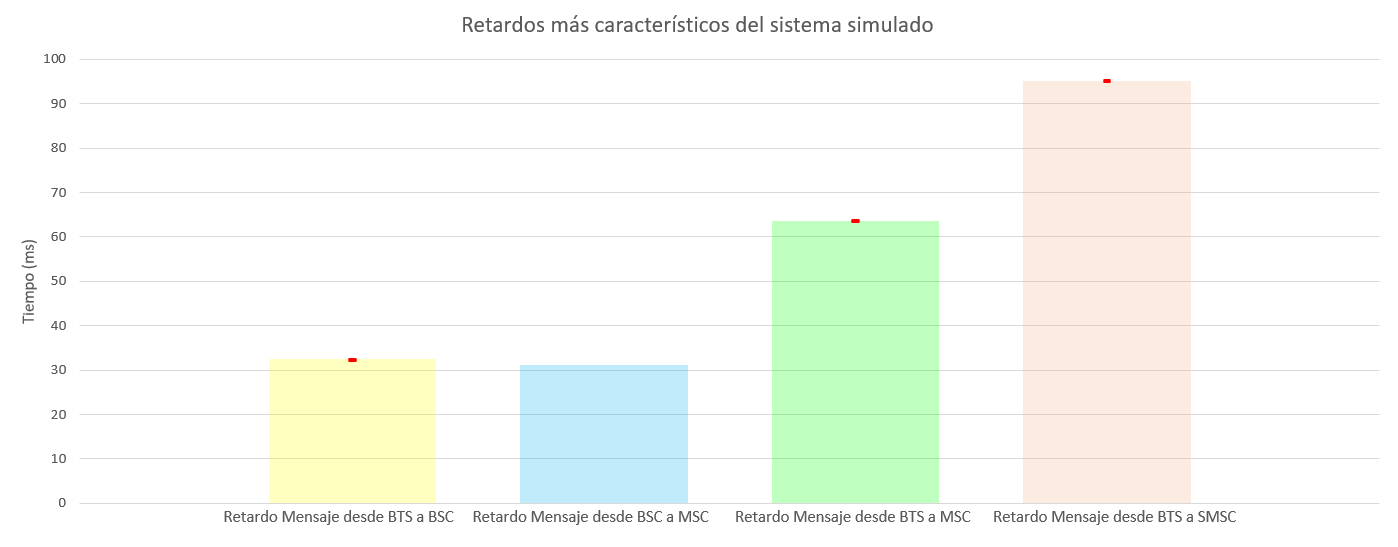
\includegraphics[width=0.75\linewidth]{message_delays.png}
					\caption{Gráfico retardos más significativos.}
					\label{f:graf_mess_del}
			\end{figure}

			\subsubsection{Una nota sobre el modelado en \texttt{COMNET III}}
				Al igual que en el caso anterior era incorrecto modelar el sistema en \texttt{COMNET III} inyectando el tráfico de manera artificial, esta situación no se produce ahora. Al estar trabajando en un contexto de conmutación de paquetes y no de circuitos no asistiremos a ningún tipo de pérdida en el \textit{backbone} de datos (recordemos que el modelo $M/D/1$ se supone con una cola de capacidad infinita). Al no tener ninguna probabilidad de bloqueo en el sistema las tasas se mantendrán intactas en todos los enlaces o lo que es lo mismo, la tasa de \texttt{SMS} resultante es igual que el agregado de todas las tasas individuales. Por ello podemos simplificar enormemente el modelado inyectando artificialmente el tráfico de los demás elementos del sistema tal y como vemos en la figura \ref{f:sms_system}.

				\begin{figure}
					\centering
					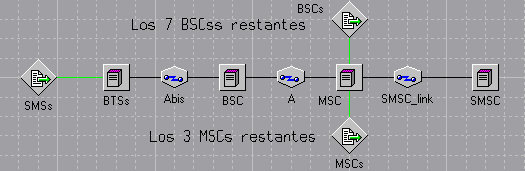
\includegraphics[width=0.5\linewidth]{sms_system.png}
					\caption{Modelo del \textit{backbone} de \texttt{SMS}.}
					\label{f:sms_system}
				\end{figure}

			\subsubsection{Comentarios finales sobre los retardos de los \texttt{SMS}}
				Una vez más, tal y como hemos hecho al estudiar las probabilidades de bloqueo de las llamadas, no hemos seguido la estructura que se desgrana del guión de la práctica. Esto no es sin embargo un acto de pura rebeldía. Sinceramente creemos que exponer nuestros cálculos seguidos del respaldo derivado de las simulaciones nos permite mantener una mayor claridad en el documento a la vez que ayuda a mantenerlo relativamente escueto y manejable.

	\section{Conclusión}
		Esperamos haber sido capaces de esclarecer tanto la base teórica que sustenta el análisis como el proceso y los resultados de la simulación que los corroboran.
		Asimismo, creemos haber enfocado aspectos sutiles de la representación de modelos y las implicaciones que pueden suponer la representación escogida. Así, debemos conocer la naturaleza del tráfico para juzgar si un modelo simplificado capturará todas las visicitudes de un sistema o si este resultará insuficiente y nos veremos obligados a trabajar con un modelo más complejo pero completo.

		En el guión de esta práctica se nos pregunta si es mejor emplear una estrategia basada en un estudio puramente teórico o si por el contrario debemos recurrir a la simulación pura. Afirmaciones categóricas como esta son tremendamente arriesgadas ya que como en muchos otros campos no creemos que una estrategia sea siempre superior a otra. A lo largo del curso nos hemos dado cuenta de cómo el análisis teórico de los sistemas de telecomunicaciones es rápido y sorprendentemente exacto pero puede carecer del empaque que proporciona una simulación. Al fin y al cabo, la simulación nos permite trabajar con una "maqueta" de un sistema real. Un punto en el que el análisis formal aventaja a la simulación es la adaptabilidad. No debemos invertir muchos recursos en modelar un sistema matemáticamente pero las simulaciones de infraestructuras complejas pueden llegar a ser muy costosas no solo en el tiempo que lleva contruir el modelo sino luego en el tiempo de ejecución de la propia simulación. Con todo, la simulación es más asequible en el sentido de que no estamos obligados a capturar las sutilezas del sistema como puede ser la inexistencia de una cola en la interfaz $A$, por ejemplo. Con todo, creemos que la simbiosis de estas dos formas de estudio es lo que de verdad nos permite llevar a cabo un análisis completo y válido pero, de tener que elegir una de las estrategias nos quedaríamos con el estudio teórico. La adaptabilidad de la que hace gala así como la mayor costumbre que tenemos, hacen que nos resulte algo más atractivo.

		En definitiva, esperamos haber realizado un buen informe en el que se plasme la gran cantidad de aspectos que hemos aprendido o en los que hemos profundizado de las infraestructuras \texttt{GSM}. Muchas gracias por su tiempo y atención.
\end{document}